\documentclass[12pt, twoside, a4paper]{report}
\pagestyle{headings}

\usepackage[latin1]{inputenc}
\usepackage[french]{babel}
\usepackage{latexsym}
\usepackage{graphics}
\oddsidemargin 1 cm
\evensidemargin 1 cm
\textwidth 15 cm

\topmargin 0 cm
\textheight 22.5 cm

\title{{\bf Projet DELTA}\\Sp�cification d'interface graphique}
\author{Batoussa MOUGAMADOU\\ Saliou NGOM\\ Vincent
BOISSIN\\ Gabriel DUPONT\\ Julien KIRSCH \\ Frederic GARCIA}
\date{IUP3-Maitrise 2002-2003\\Informatique et Math�matiques}

\usepackage[dvips]{graphicx}

\begin{document}
\maketitle
\tableofcontents

\chapter{Pr�ambule}
Pour la repr�sentation des zoning, nous avons choisi d'adopter une
convention pour les couleurs des textes utilis�s.
\begin{flushleft}
\scalebox{0.5}{\includegraphics{../eps/template.eps}}\\
\end{flushleft}







\chapter{Introduction}

L'interface graphique de l'application web que nous allons d�velopp�e
s'appuie sur les derni�res technologies d'outils web.
Ce qui offre les avantages d'une norme internationale reconnue, d'une
compatibilit� avec tous les environnements Java, y compris les
navigateurs web.
L'utilisation de ces outils sont dues � la n�cessit� d'utiliser
une ref�rence commune de composants graphiques r�utilisables et ceci
dans un but technique et surtout pratique.
Ces technologies fournissent un code simple qui permet de cr�er une
interface tr�s pratique � l'aide des outils de cr�ation d'interface
graphique.

\section*{Objectifs }

\begin{itemize}
\item R�utisabilit�
\\
L'interface va former des briques pour son ind�pendance et sa
r�utilisabilit�.
On veut assurer la compl�te r�utilisabilit� de l'interface graphique
avec le moins de retouches de code source. 
\\
\item Simplicit�
\\
L'utilisation de notre interface par un autre d�veloppeur d'interface
ou un utilisateur qui construit lui-m�me une interface sera simple et
rapide.
Les balises vont communiquer entre elles par des messages bien
formalis�es.
Ces balises seront interchangeables. Si une partie de l'interface doit
changer pour cause d'une mise � jour o� d'ajout de fonctionnalit�, il
suffira de remplacer la balise obsol�te.
\\
\item Portabilit�
\\
L'interface sera �crit en JSP,HTML. Or ces technologies sont
maintenant tr�s largement portables.Ils sont utilisables aussi bien
sous Linux ou n'importe quel autre syst�me supportant java.
L'interface qui sera d�velopp�e aura le m�me aspect sur toutes les
platesformes.
On ne peut r�ver mieux en mati�re de portabilit�.
\\
\item Extensibilit�
\\
Les composants utilis�s par notre interface graphique seront
susceptibles d'�tre enrichis � volont�.
Donc il ne s'agit pas de r�ecrire une interface pour chaque nouveau
code.
\\
\item Normalisation:
\\
Notre interface est fond�e sur la norme ISO qu'est JSP et HTML et qui
sont des standards de l'industrie informatique.
Ceci garantit sa compatibilit� avec tous les environnements
d'exploitation et les navigateurs web comme Netscape
Navigator,Netscape Communicator, Internet Explorer ou Mozilla.
\end{itemize} 












\chapter{La charte graphique}
Nous proposons dans ce projet de respecter une charte graphique que
toutes les pages de l'application vont respecter. Cette charte
repr�sente plus concr�tement un mod�le de page.\\
En voici un patron :
\begin{flushleft}
\scalebox{0.6}{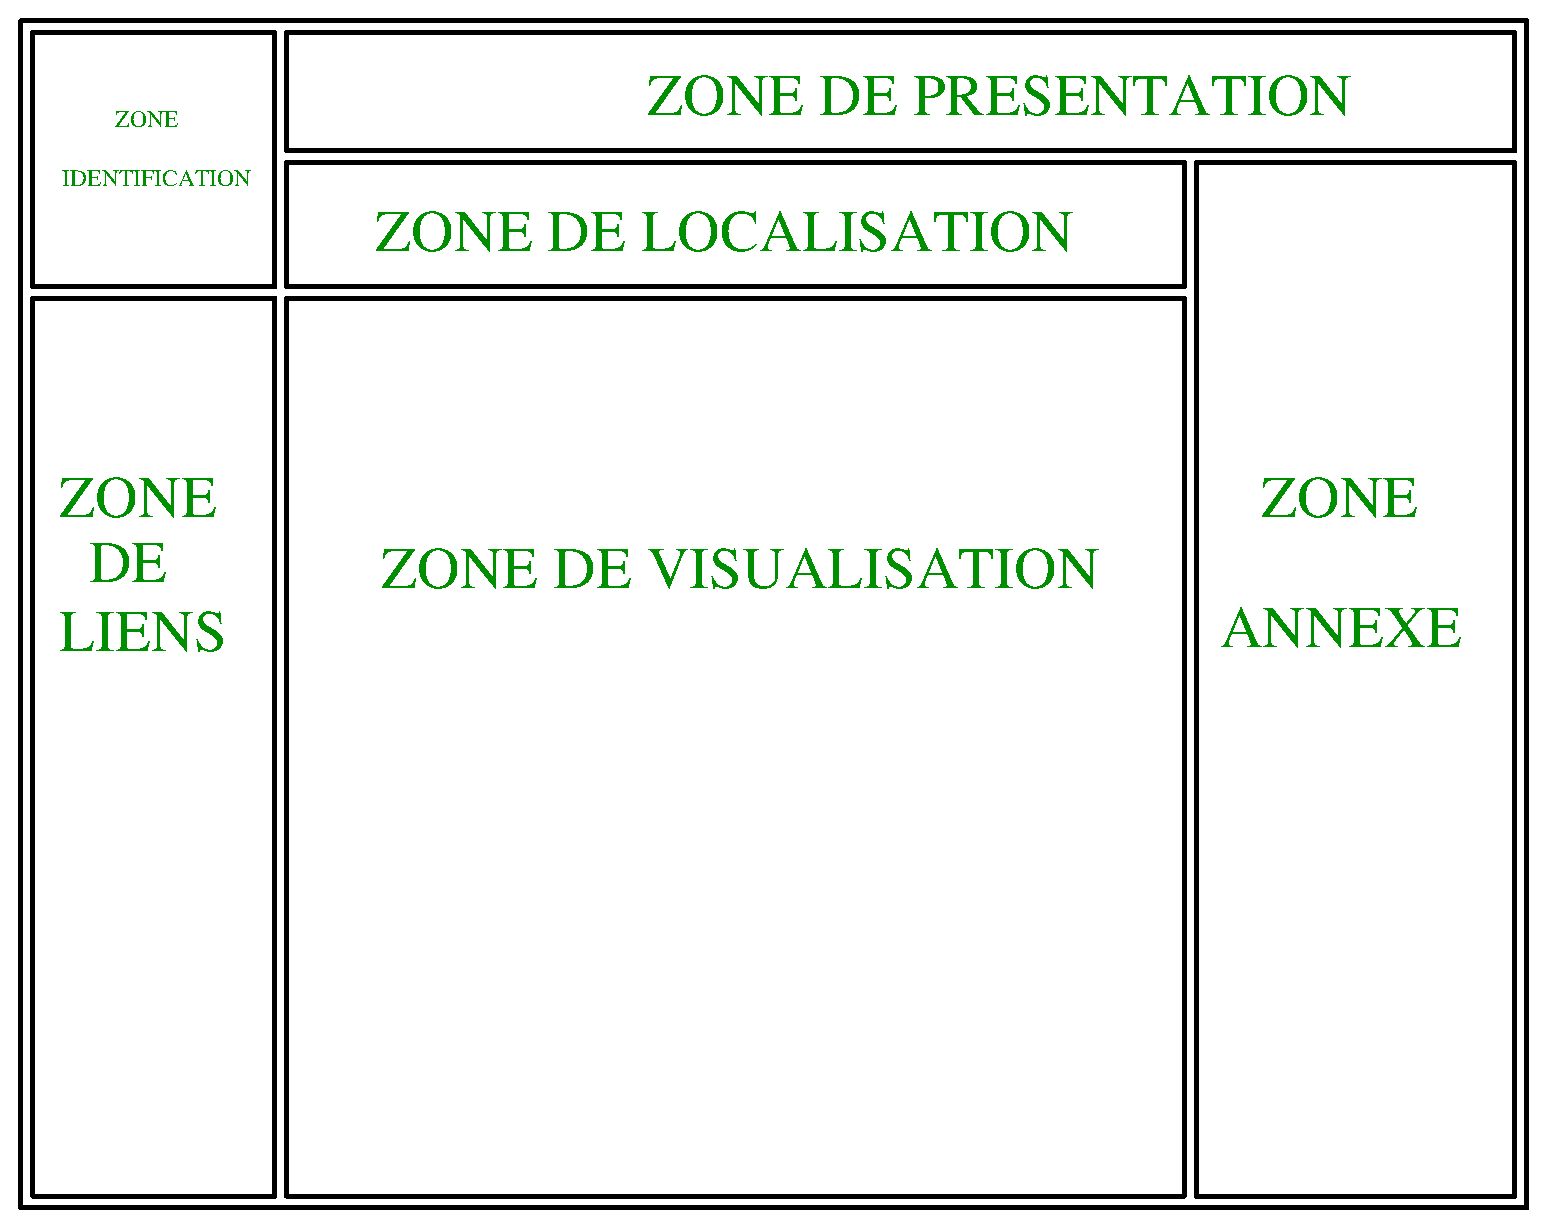
\includegraphics{../eps/charte.eps}}\\
\end{flushleft}


\chapter{La zone de pr�sentation}
La zone de pr�sentation est compos�e du logo de la soci�t� Delta,
c'est-�-dire nous, ainsi que du titre de l'application et de la date
et heure courante. Cette zone est dynamique quant � la date et heure courante.  
\begin{flushleft}
\scalebox{0.6}{
\includegraphics{../eps/logo.eps}}\\
\end{flushleft}


\chapter{La zone d'identification}
LA zone d'identification est la zone permettant � un utilisateur
d'interagir avec l'application.\\Cette zone a deux �tats :
\begin{itemize}
\item ``Login et Mot de passe'' lorsque l'utilisateur est un consultant 
\item Le login de la personne identifi� sinon
\end{itemize}
\begin{flushleft}
\scalebox{0.6}{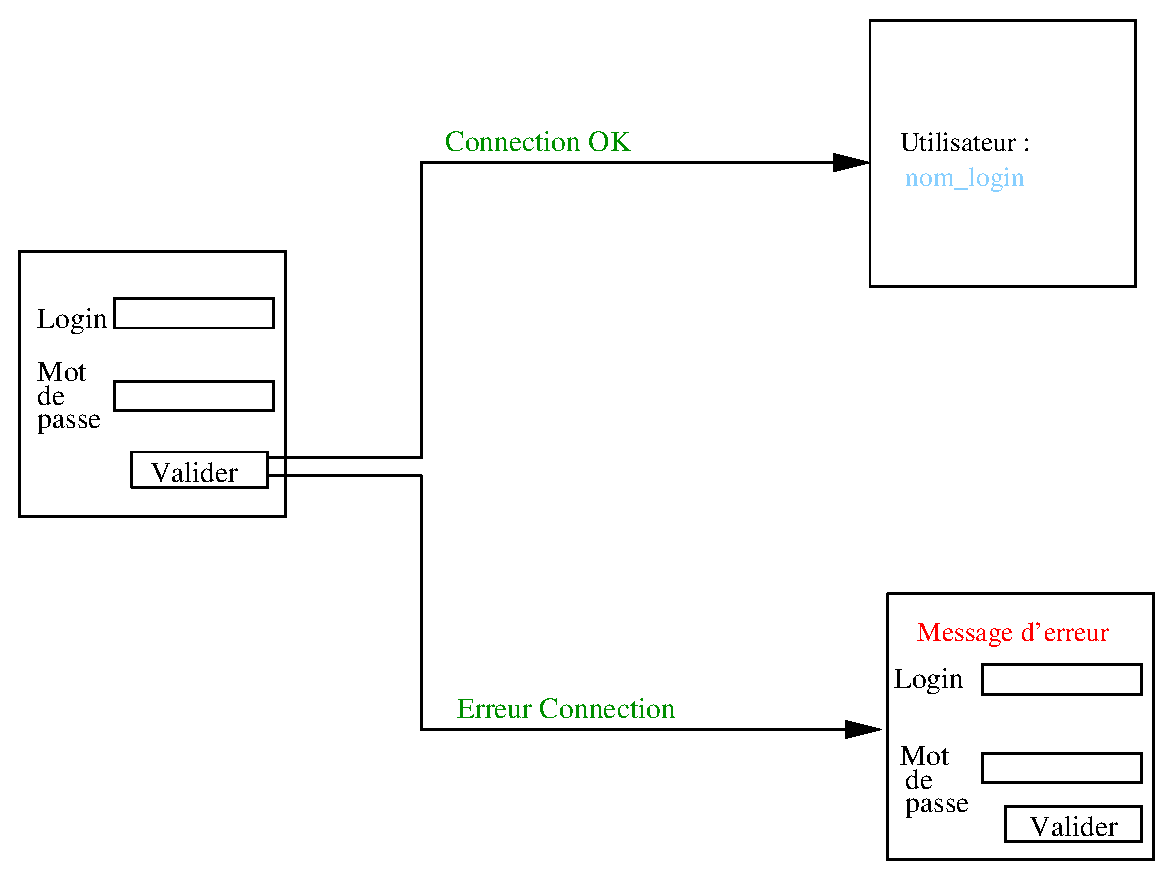
\includegraphics{../eps/login.eps}}\\
\end{flushleft}


\chapter{La zone de localisation}

La zone de localisation permet � l'utilisateur de l'application de
savoir � chaque instant dans quel �tat se trouve l'application. Cette
zone est repr�sent� par des onglets (non cliquables).Par
exemple, si l'utilisateur est en train de consulter un exercice,
l'onglet se trouve sur {\it Compte}.\\
Cependant, cette zone contient plus ou moins de champs selon la nature
de l'utilisateur. En effet, un consultant ne pourra pas faire plus que
de consulter des projets ou TD.\\
Voici un aper�u des diff�rents �tats de la zone de localisation selon l'utilisateur.

\begin{flushleft}
\scalebox{0.6}{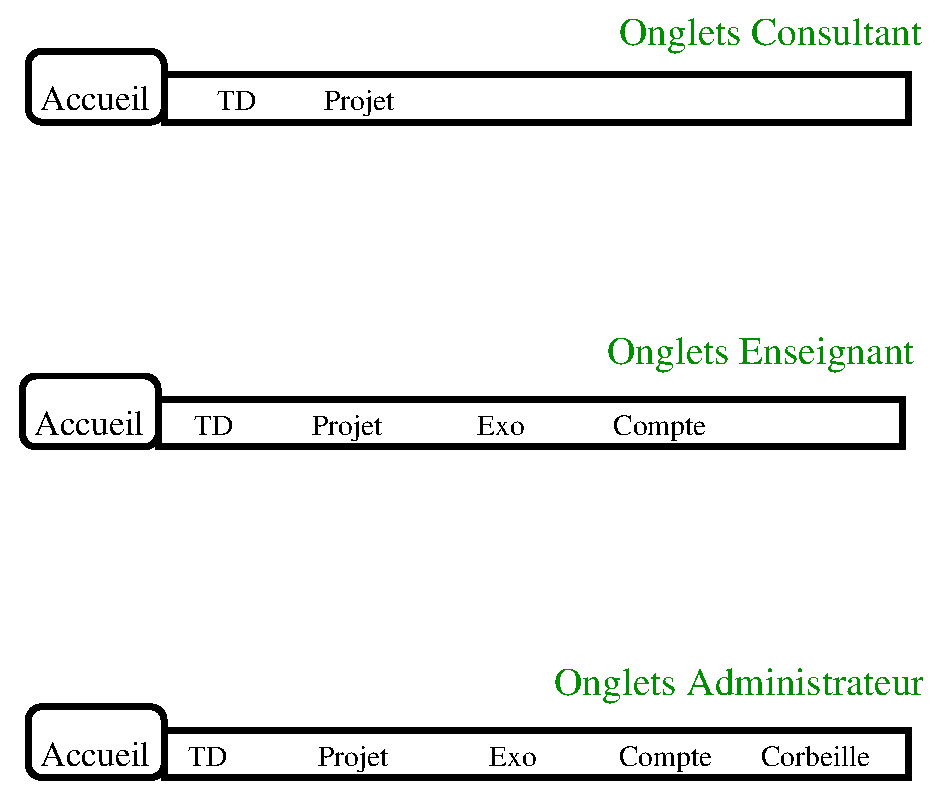
\includegraphics{../eps/onglets.eps}}\\
\end{flushleft}


\chapter{La zone des liens}

La zone des liens est une zone contenant les diff�rents liens
principaux de l'application. Cette zone est statique et diff�re selon
l'utilisateur. 
Par exemple, on peut voir apparaitre le lien {\it se d�connecter} pour
l'enseignant et l'administrateur qui
n'aurait aucune utilit� pour le consultant.\\
De m�me, quant � la recherche, selon l'utilisateur, le(s) type(s) de
donn�e(e) pouvant �tre recharch�(s) sera(ont)
diff�rent(s). L'utilisateur pourra effectuer une recherche multiple,
c'est-�-dire par exemple, les TD et projets simultan�ment.\\
Pour le consultant, apparaissent des liens de th�me tel que {\it Java}
qui repr�sente en fait une recherche compl�te avec comme mots cl�s Java.
\begin{flushleft}
\scalebox{0.6}{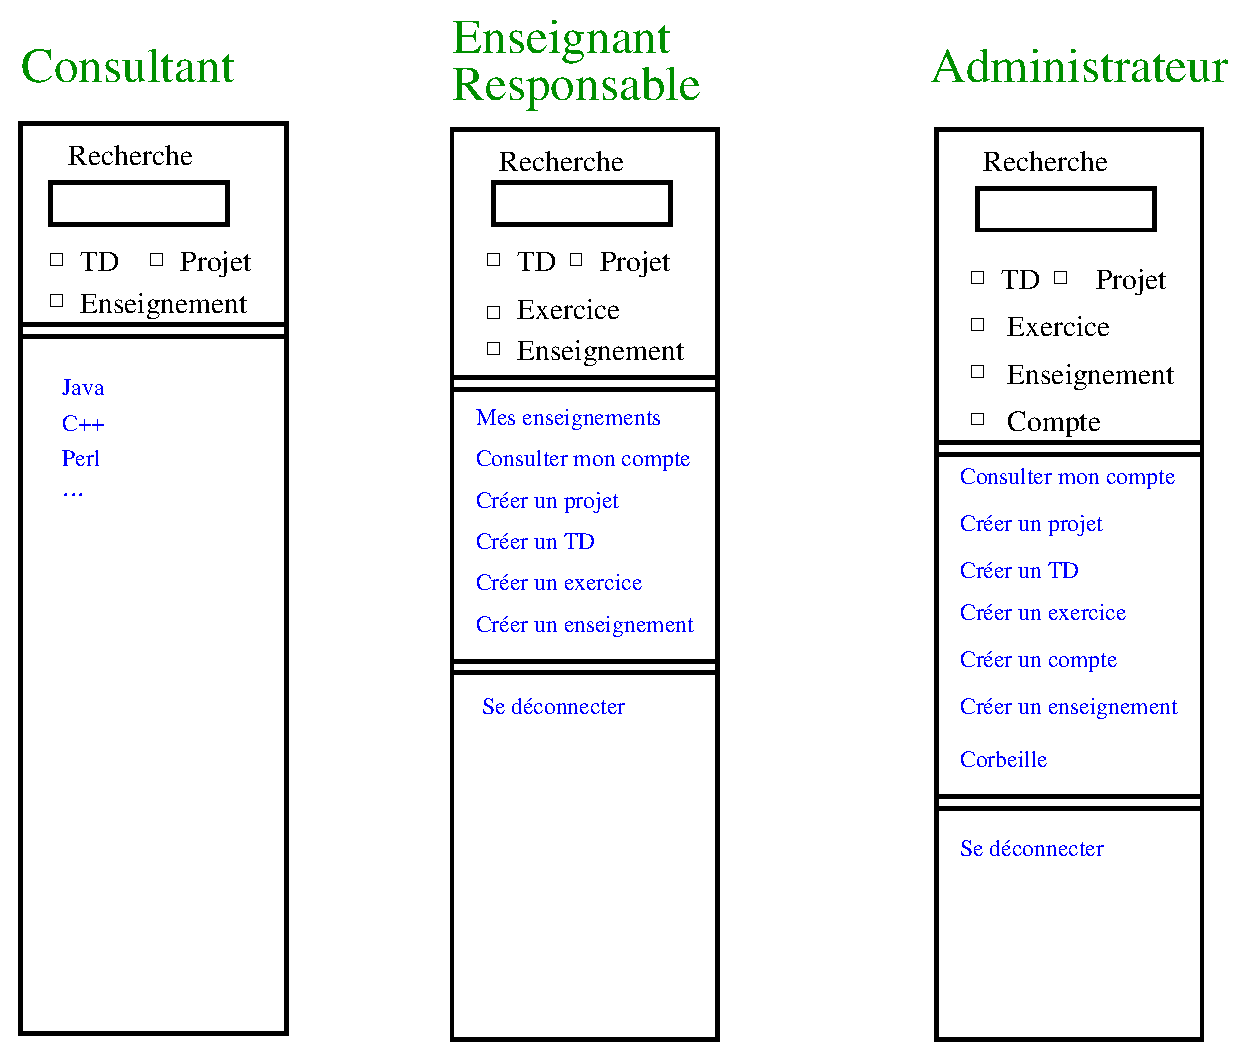
\includegraphics{../eps/Liens.eps}}\\
\end{flushleft}




\chapter{La zone annexe}
LA zone annexe va de pair avec la zone de visualisation (voir plus
bas). En effet, cette zone contient des actions,g�n�ralement
repr�sent�es par des liens, ayant une int�raction direct avec les
donn�es de la zone de visualisation. Par exemple, si l'utilisateur
consulte un projet, apparaitra sur la zone annexe un lien {\it
T�l�charger} qui permattra de t�l�charger le projet consult�.\\
Nous verrons avec la pr�sentation de la zone de visualisation
l'avantage de la zone annexe.

\chapter{La zone de visualisation}
\section{Pr�sentation}
La zone de visualisation est la zone la plus importante de
l'application. En effet, c'est sur cette zone que s'afficheront les
diff�rentes pages. Par exemple, lors de la visualisation d'un projet,
la version en HTML du projet apparaitra dans la zone de visualisation.\\ 
Voici une description des pages apparaissant dans
cette zone.\newpage
\section{Mes enseignements}
Voici les diff�rentes �tapes lorsque l'enseignant clique sur {\it Mes
enseignements}.\\ Commen�ons par la sp�cification de la premi�re page apparaissant.
\subsection{Page principale}
\begin{flushleft}
\scalebox{0.6}{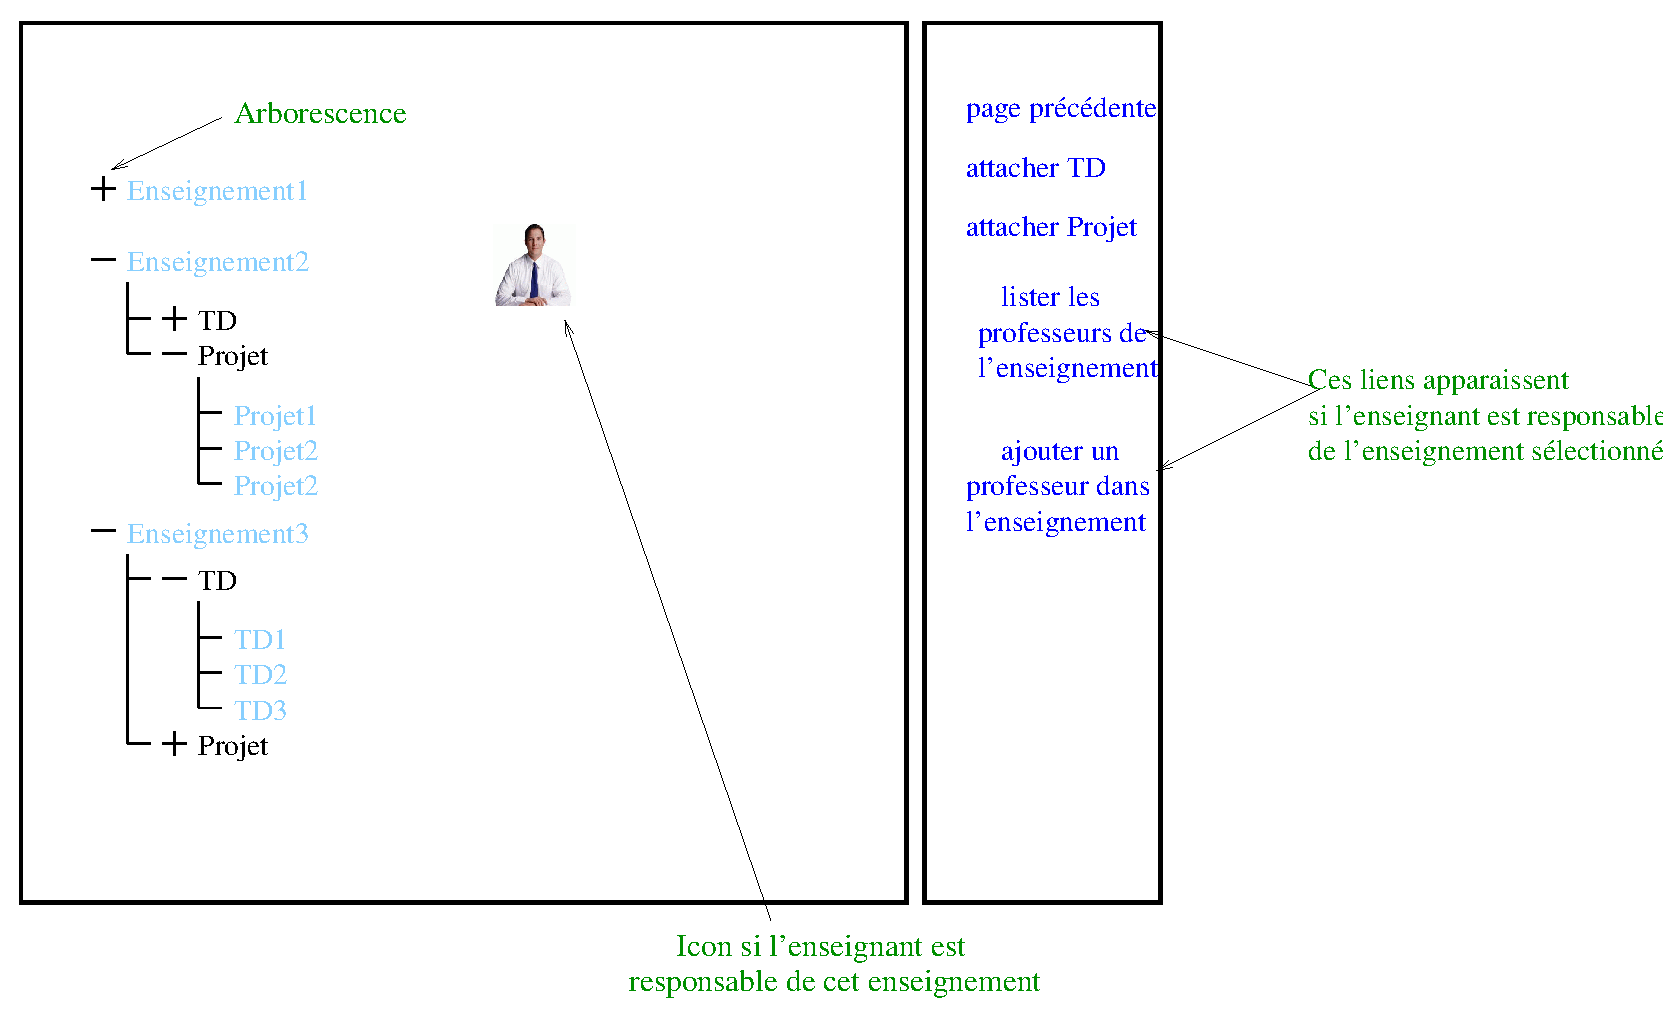
\includegraphics{../eps/MesEnseignements.eps}}\\
{\it Premi�re page de Mes enseignements}
\end{flushleft}
Cette page repr�sente un listing de tous les enseignements dans
lesquels l'enseignant connect� appartient. Si l'enseignant
est responsable d'un des enseignements, alors une icon apparait � c�t�
de l'enseignement.\\De plus, si l'enseignant selectionne un
enseignement dans lequel il est responsable, de nouvelles
fonctionnalit�s (liens) appraissent dans la zone annexe.
\newpage

Lors de la consultation de ses enseignements, l'enseignant peut
attacher un projet � un de ses enseignements.
\begin{flushleft}
\scalebox{0.5}{\includegraphics{../eps/Attacher1Projet.eps}}\\
{\it Page principale de l'attachement d'un projet}
\end{flushleft}
Lorsque l'enseignant choisit d'attacher un projet pr�sent dans la
base de l'apllication, apparait une nouvelle fen�tre contenant la liste
des projets class�s par enseignements.
\begin{flushleft}
\scalebox{0.5}{\includegraphics{../eps/AttacherProjetExistant.eps}}\\
{\it Liste des projets pouvant �tre attach�s}
\end{flushleft}
\newpage
\subsection{Attacher un TD}
Lors de la consultation de ses enseignements, l'enseignant peut
attacher un TD � un de ses enseignements.
\begin{flushleft}
\scalebox{0.5}{\includegraphics{../eps/Attacher1TD.eps}}\\
{\it Page principale de l'attachement d'un TD}
\end{flushleft}

Lorsque l'enseignant choisit d'attacher un TD pr�sent dans la
base de l'application, apparait une nouvelle fen�tre contenant la liste
des TD class�s par enseignements.
\begin{flushleft}
\scalebox{0.5}{\includegraphics{../eps/AttacherTDExistant.eps}}\\
{\it Liste des TD pouvant �tre attach�s}
\end{flushleft}

\subsection{Liste des professeurs de l'enseignement}
Le responsable d'un enseignement a la possibilit� de lister tous les
enseignants de son enseignement. Ainsi, il peut g�rer les droits dans
son enseignement c'est-�-dire ajouter ou retirer les droits � des
enseignants pour acc�der � leur enseignement. 
\begin{flushleft}
\scalebox{0.5}{\includegraphics{../eps/ListingProfD1Enseignement.eps}}\\
{\it Liste des professeurs de l'enseignement}
\end{flushleft}

\begin{flushleft}
\scalebox{0.5}{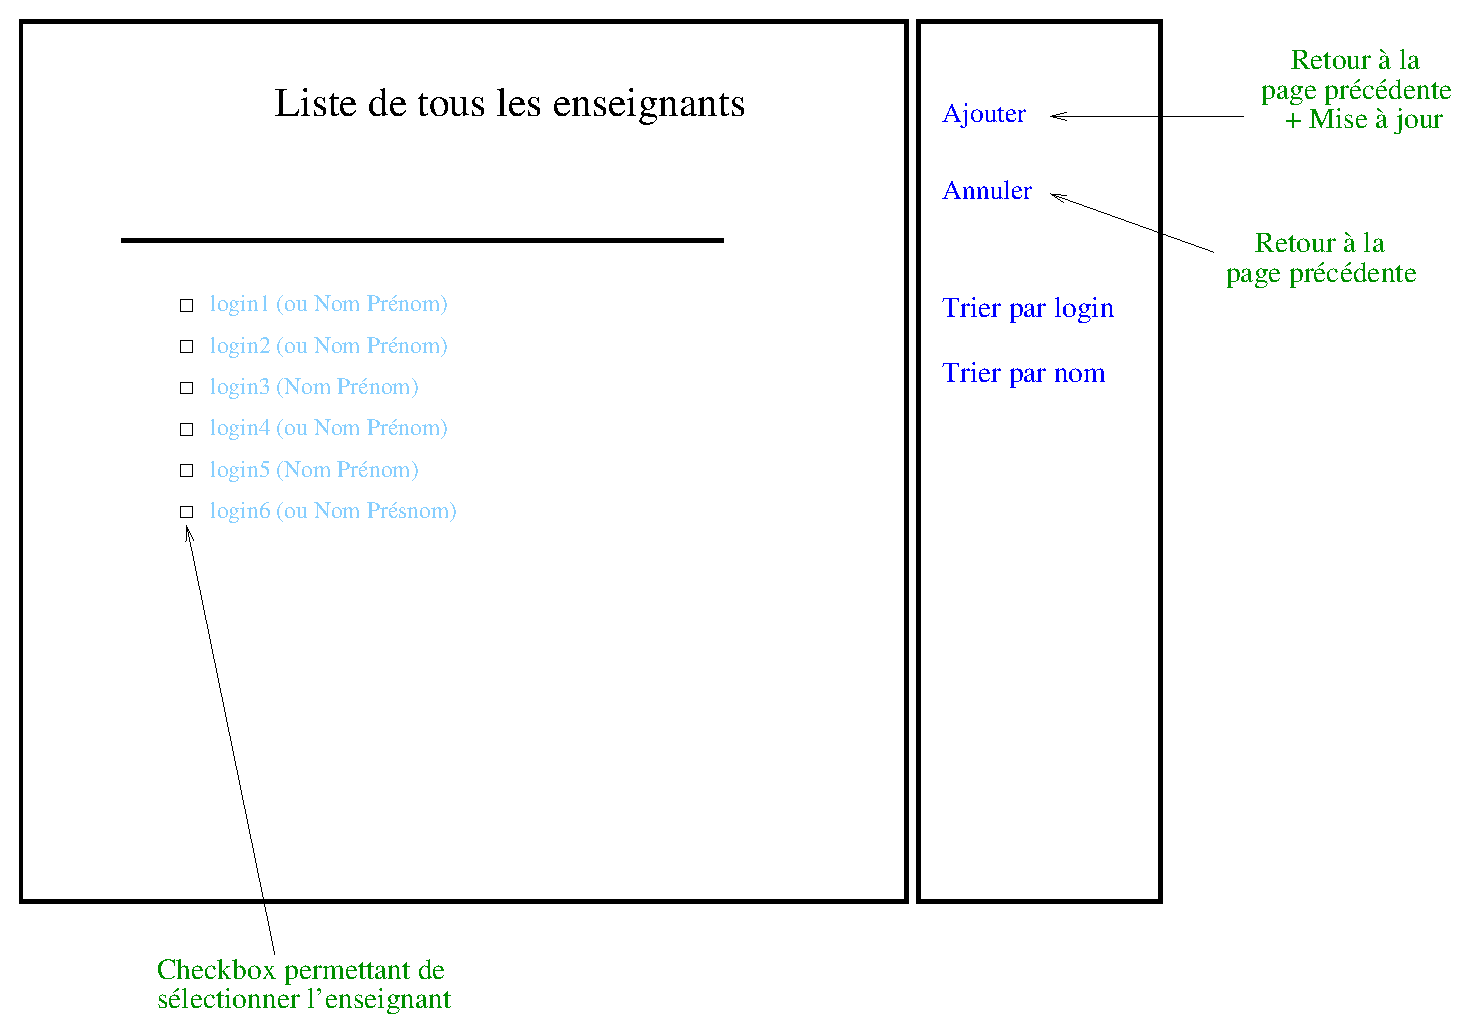
\includegraphics{../eps/AjoutD1NouveauProf.eps}}\\
{\it Liste de tous les professeurs de la base sauf ceux de l'enseignement}
\end{flushleft}












\section{Consulter son compte}

L'utilisateur a la possiblit� de consulter son compte et
�ventuellement de modifier ses param�tres personnels.
Toutefois, la modifcation du login n'est pas autoris� pour des raisons
de coh�rence dans la base.
\begin{flushleft}
\scalebox{0.5}{\includegraphics{../eps/compteConsulter.eps}}\\
{\it Fen�tre de consultation de son compte}
\end{flushleft}

\begin{flushleft}
\scalebox{0.5}{\includegraphics{../eps/compteModifier.eps}}\\
{\it Modifcation des param�tres}
\end{flushleft}

\begin{flushleft}
\scalebox{0.5}{\includegraphics{../eps/compteModifierMDP.eps}}\\
{\it Modifcation du mot de passe}
\end{flushleft}

\begin{flushleft}
\scalebox{0.5}{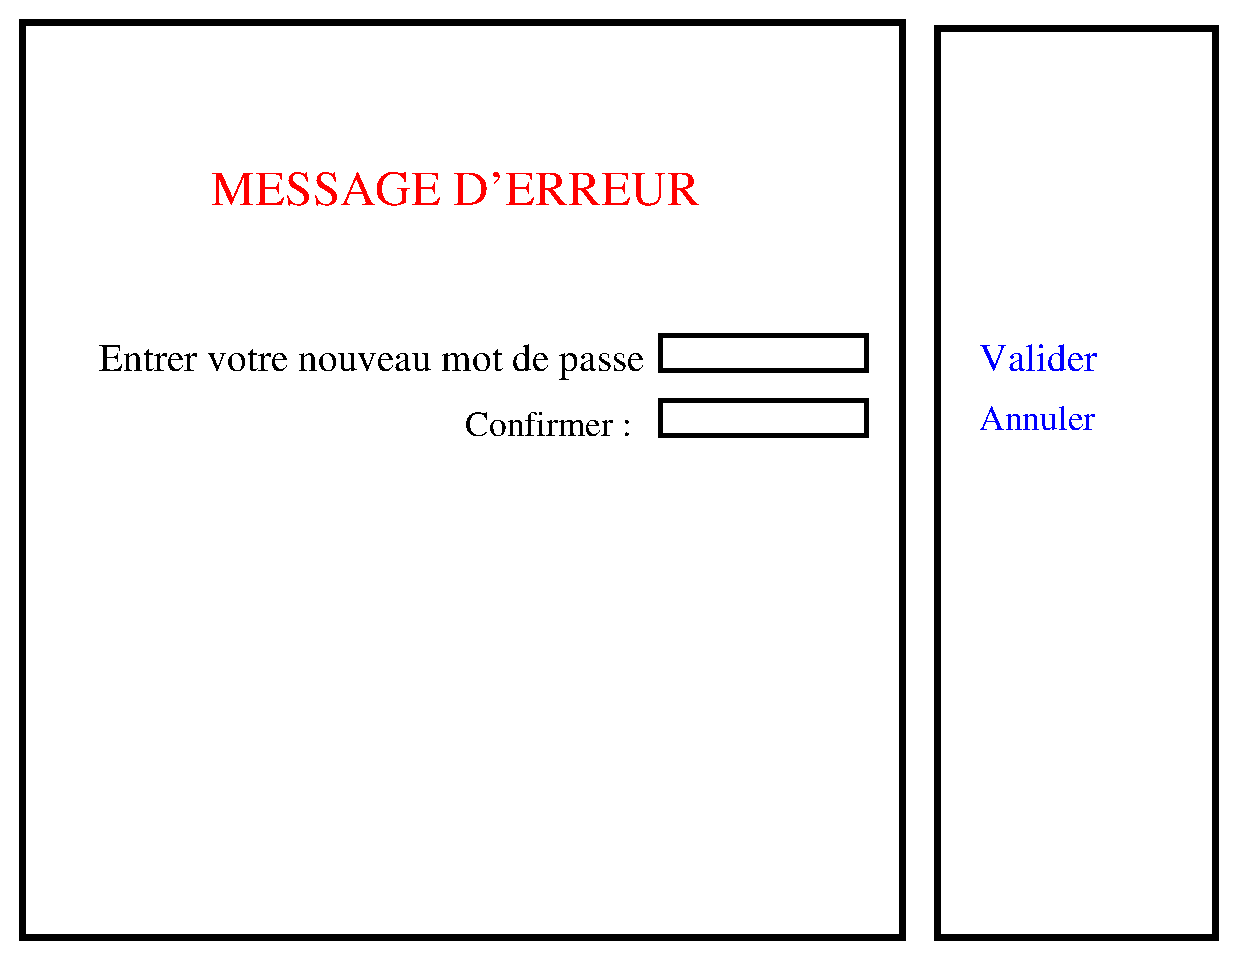
\includegraphics{../eps/compteModifierMDPErreur.eps}}\\
{\it Modifcation incorrect}
\end{flushleft}




\section{Cr�er un projet}
\subsection{Page principale}
Nous allons d�tailler dans cette partie le sc�nario de cr�ation d'un projet.
L'enseignant cr�e un projet en cliquant sur le lien {\it Cr�er un projet} dans la zone de lien.
Il existe deux mani�res de cr�er un projet:
\begin{itemize}
\item Soit il reprend un projet qui existe dans la base : lien {\it � partir d'un projet existant dans la base}
\item Soit il en cr�e un nouveau : lien {\it un nouveau projet}
\end{itemize}

\begin{flushleft}
\scalebox{0.5}{\includegraphics{../eps/CreerProjetMain.eps}}\\
{\it Page principale}
\end{flushleft}

\subsection{A partir d'un ancien}
L'enseignant doit s�lectionner un projet dans la base.
Il s�lectionne le projet � l'aide d'une arborescence des enseignements.
Il peut lister les projets des enseignements en cliquant sur les noeuds des enseignements.
Un simple clic sur les projets ouvre l'�diteur pour la cr�ation du nouveau projet.
\begin{flushleft}
\scalebox{0.5}{\includegraphics{../eps/CreerProjAncien_Listing.eps}}\\
{\it Liste des projets existants dans la base tri�s par enseignements}
\end{flushleft}
\newpage
\subsection{Nouveau projet}
Il existe deux mani�res de cr�er un nouveau projet:
\begin{itemize}
\item Soit l'enseignant importe un fichier XML depuis son compte.
Dans ce cas un navigateur permet � l'enseignant d'importer le fichier.
\item Soit il �dite directement le projet dans l'�diteur de bord.
\end{itemize}

\begin{flushleft}
\scalebox{0.5}{\includegraphics{../eps/CreerNewProjMain2.eps}}\\
{\it Page de cr�ation d'un projet} 
\end{flushleft}
\newpage
\subsection{Editeur de bord}
L'enseignant utilise pour la saisie du projet l'�diteur embarqu�, dans la zone de visualisation.

Il existe deux mani�res de r�diger le projet.
\begin{flushleft}
\scalebox{0.5}{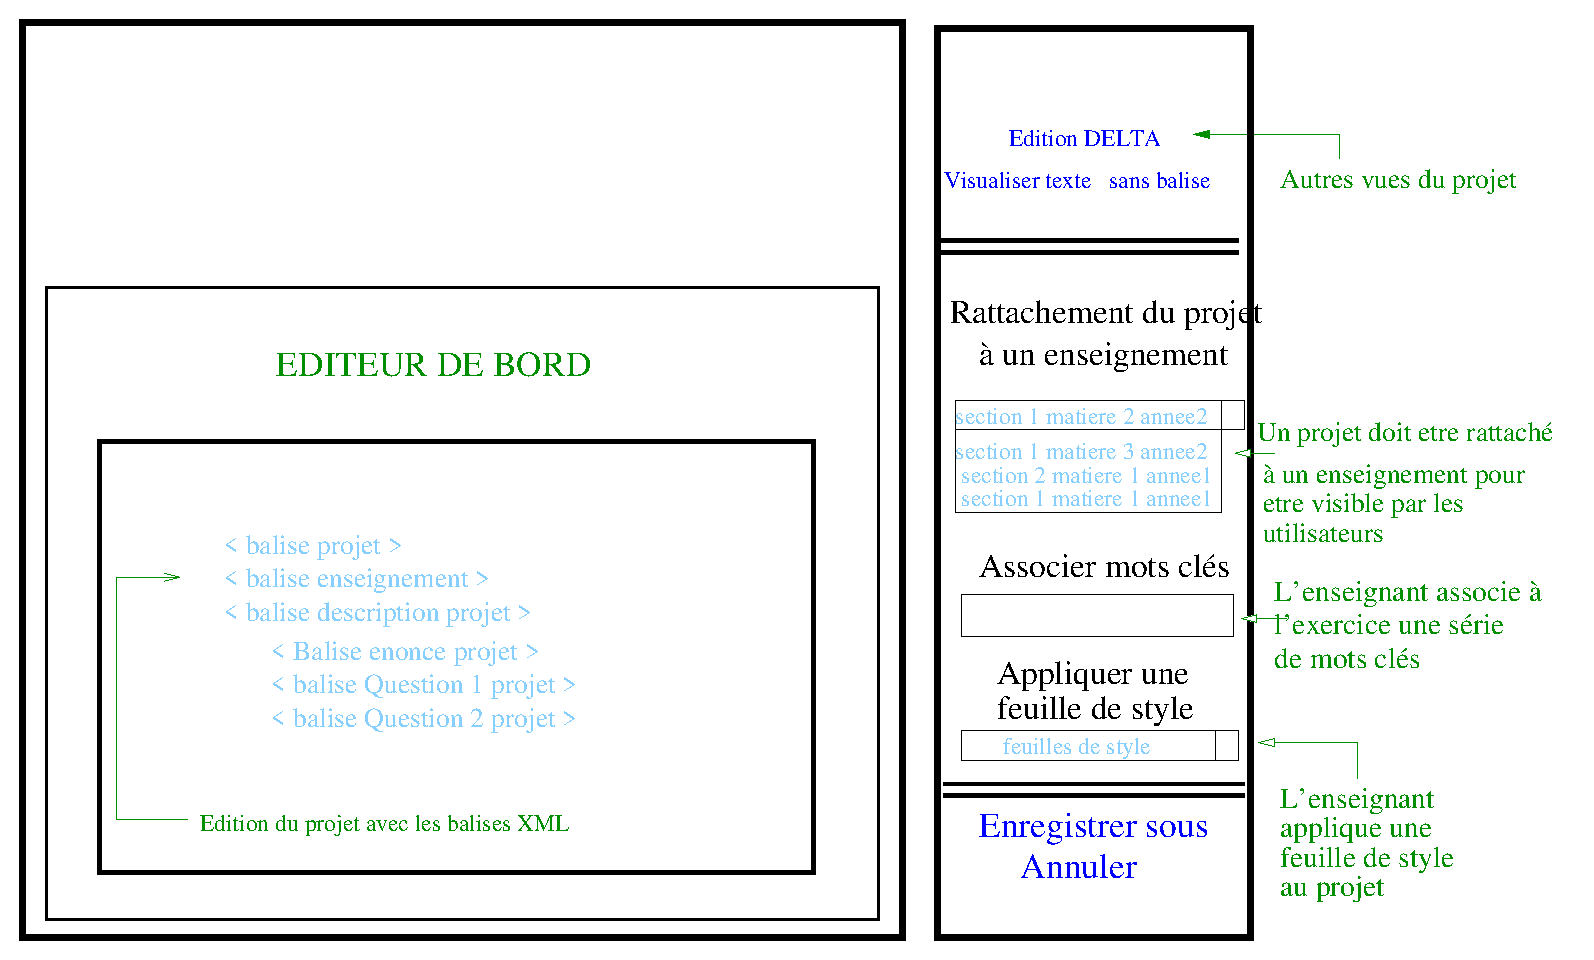
\includegraphics{../eps/projetEditionBalise.eps}}\\
{\it L'enseignant saisie le projet directement en XML}
\end{flushleft}

\begin{flushleft}
\scalebox{0.5}{\includegraphics{../eps/projetEditionSansBalise.eps}}\\
{\it L'enseignant r�dige son projet en mode texte simple (WYSIWYG)}
\end{flushleft}

Une fois le projet saisi, l'enseignant peut rattacher le projet � un enseignement.
Ainsi, le projet sera diffus� dans l'intranet dans les enseignements rattach�s.
Si l'enseignant ne rattache pas le projet � un enseignment, le projet
est stock� dans une zone temporaire.
Les consultants n'auront alors pas acc�s � ce projet.

Une fois le projet r�dig� l'enseignant l'enregistre dans la base :
lien {\it Enregistrer}




\section{Cr�er un TD}
\subsection{Page principale}
Nous allons d�tailler dans cette partie le sc�nario de cr�ation d'un TD.
L'enseignant cr�e un TD en cliquant sur le lien {\it Cr�er un TD} dans la zone de lien.
Il existe deux mani�res de cr�er un TD:
\begin{itemize}
\item Soit il reprend un TD qui existe dans la base : lien {\it � partir d'un TD existant dans la base}
\item Soit il en cr�e un nouveau : lien {\it un nouveau TD}
\end{itemize}

\begin{flushleft}
\scalebox{0.5}{\includegraphics{../eps/CreerTDMain.eps}}\\
{\it Fen�tre principale}
\end{flushleft}

\subsection{A partir d'un ancien}
L'enseignant doit s�lectionner un TD dans la base.
Il s�lectionne le TD dans le navigateur.
Il peut lister les TDs des enseignements en cliquant sur les noeuds des enseignements.
\begin{flushleft}
\scalebox{0.5}{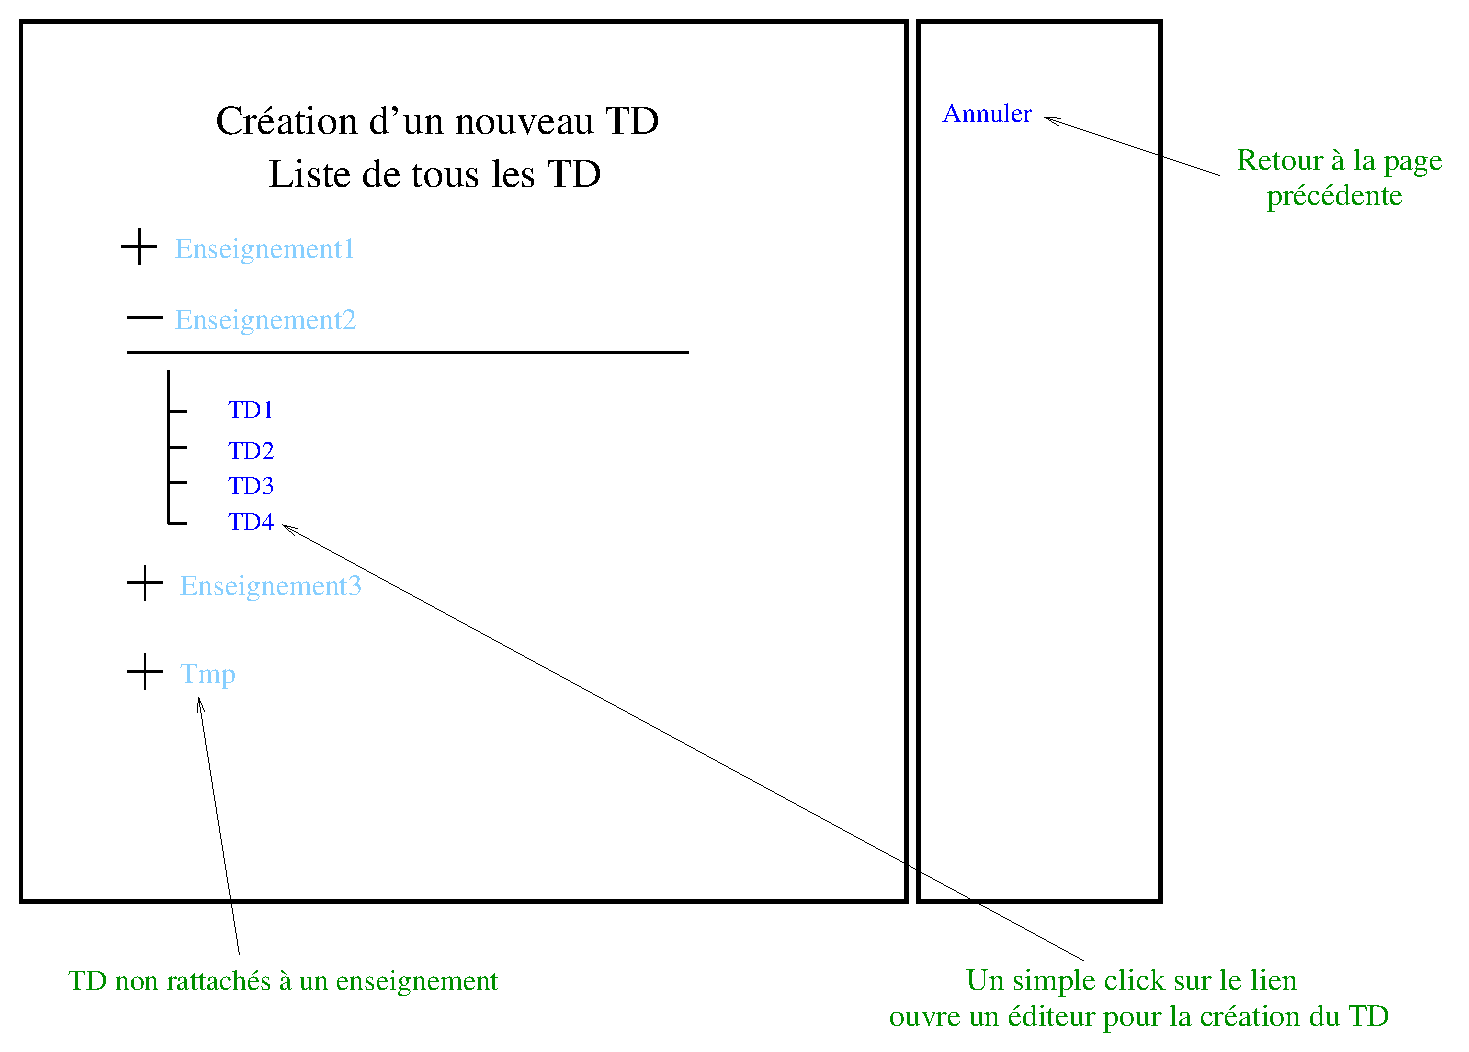
\includegraphics{../eps/CreerTDAncien_Listing.eps}}\\
{\it Listing des TD existants dans la base, tri�s par enseignements}
\end{flushleft}
\newpage
\subsection{Nouveau TD}
Il existe deux mani�res de cr�er un nouveau TD:
\begin{itemize}
\item Soit l'enseignant importe un fichier XML depuis son compte.
\item Soit il �dite directement le TD dans l'�diteur de bord.
\end{itemize}

\begin{flushleft}
\scalebox{0.5}{\includegraphics{../eps/CreerNewTDMain2.eps}}\\
{\it Page principale lors de la cr�ation d'un nouveau TD}
\end{flushleft}

\subsection{Editeurs de bord}
Plusieurs vues sont propos�es � l'enseignant pour �diter son TD.
\begin{itemize}
\item La vue Delta
\item Le fichier XML avec les balises.
\item Une version texte sans balise XML.
\end{itemize}

L'enseignant utilise pour la saisie du TD l'�diteur embarqu�, dans la zone de visualisation.

Il existe trois mani�res d'�crire le TD.


\begin{flushleft}
\scalebox{0.5}{\includegraphics{../eps/tdEditionBalise.eps}}\\
{\it L'enseignant saisie le TD soit directement en XML soit en mode texte}
\end{flushleft}

\begin{flushleft}
\scalebox{0.5}{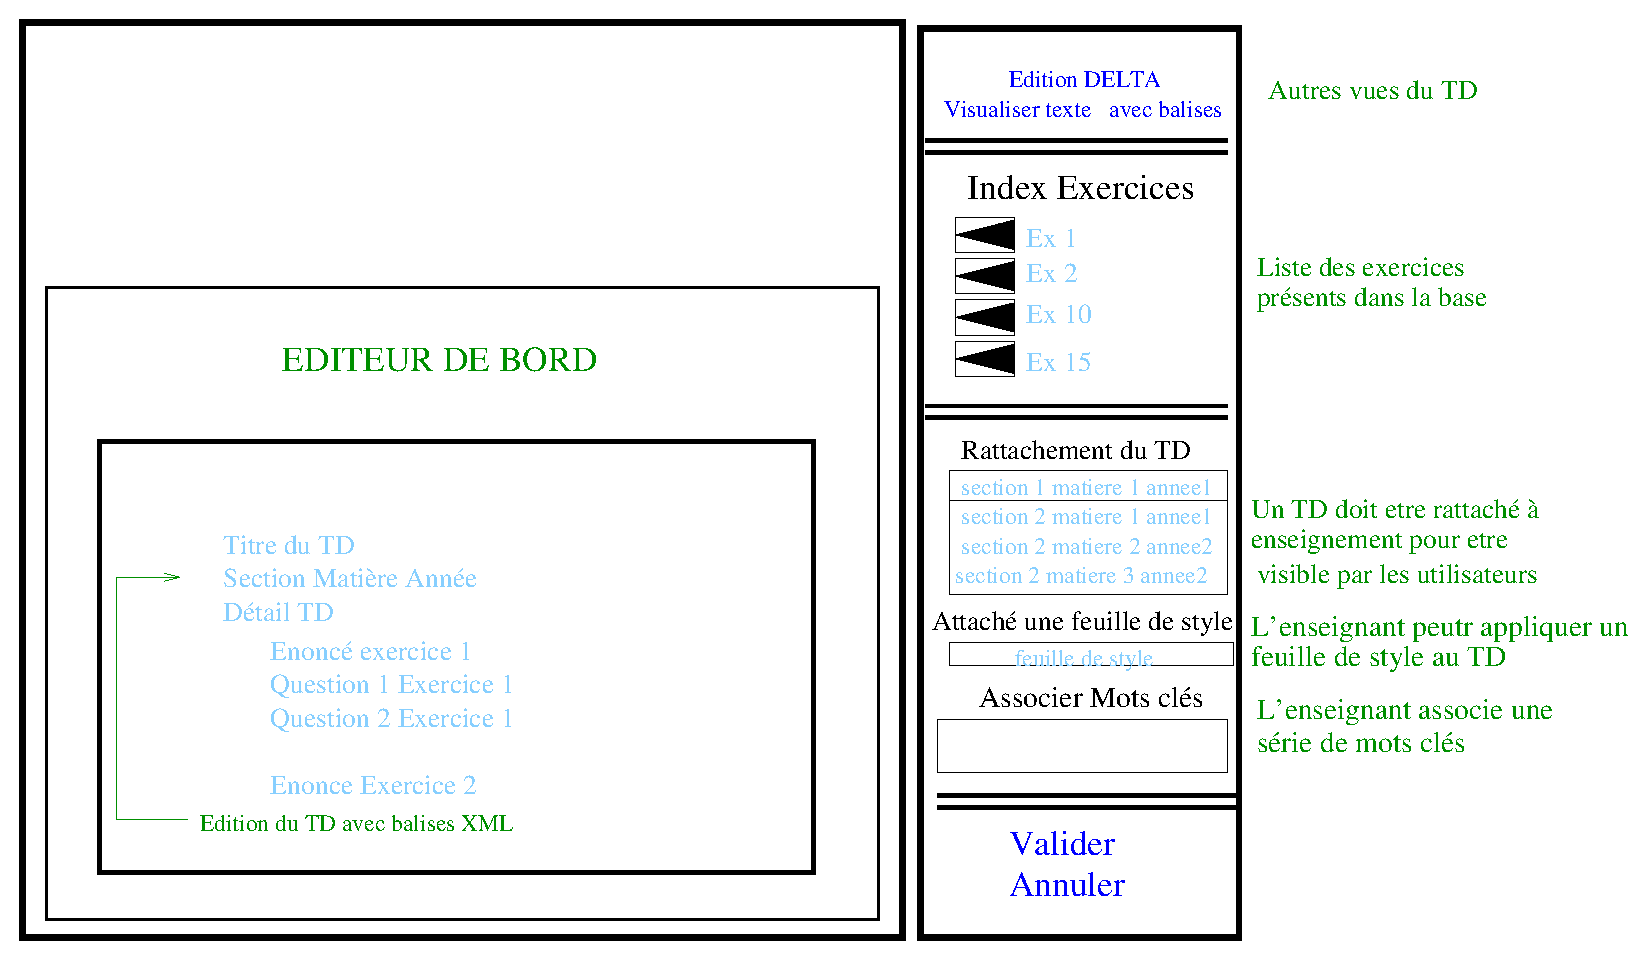
\includegraphics{../eps/tdEditionSansBalise.eps}}\\
\end{flushleft}
\newpage
La derni�re propose� est la  vue Delta. Cette vue consiste � lister le contenu du TD courant dans la zone de visualisation.
Dans la zone annexe, l'enseignant a acc�s � la liste des exercices qui existent dans la base.
Depuis l'index des exercices, l'enseignant s�lectionne un exercice et l'ajoute au TD avec la fl�che gauche.
Il peut modifier l'ordre des exercices � l'int�rieur du TD avec les deux fl�ches (Haut Bas)
Il peut �galement retirer un exercice du TD qu'il construit avec la fl�che droite.
Une fois le TD construit, pour diffus� le TD il doit le rattacher � un enseignement.
S'il ne le rattache pas, le TD ne sera pas visible pour les
consultants et sera stock� dans un r�pertoire temporaire.
\begin{flushleft}
\scalebox{0.5}{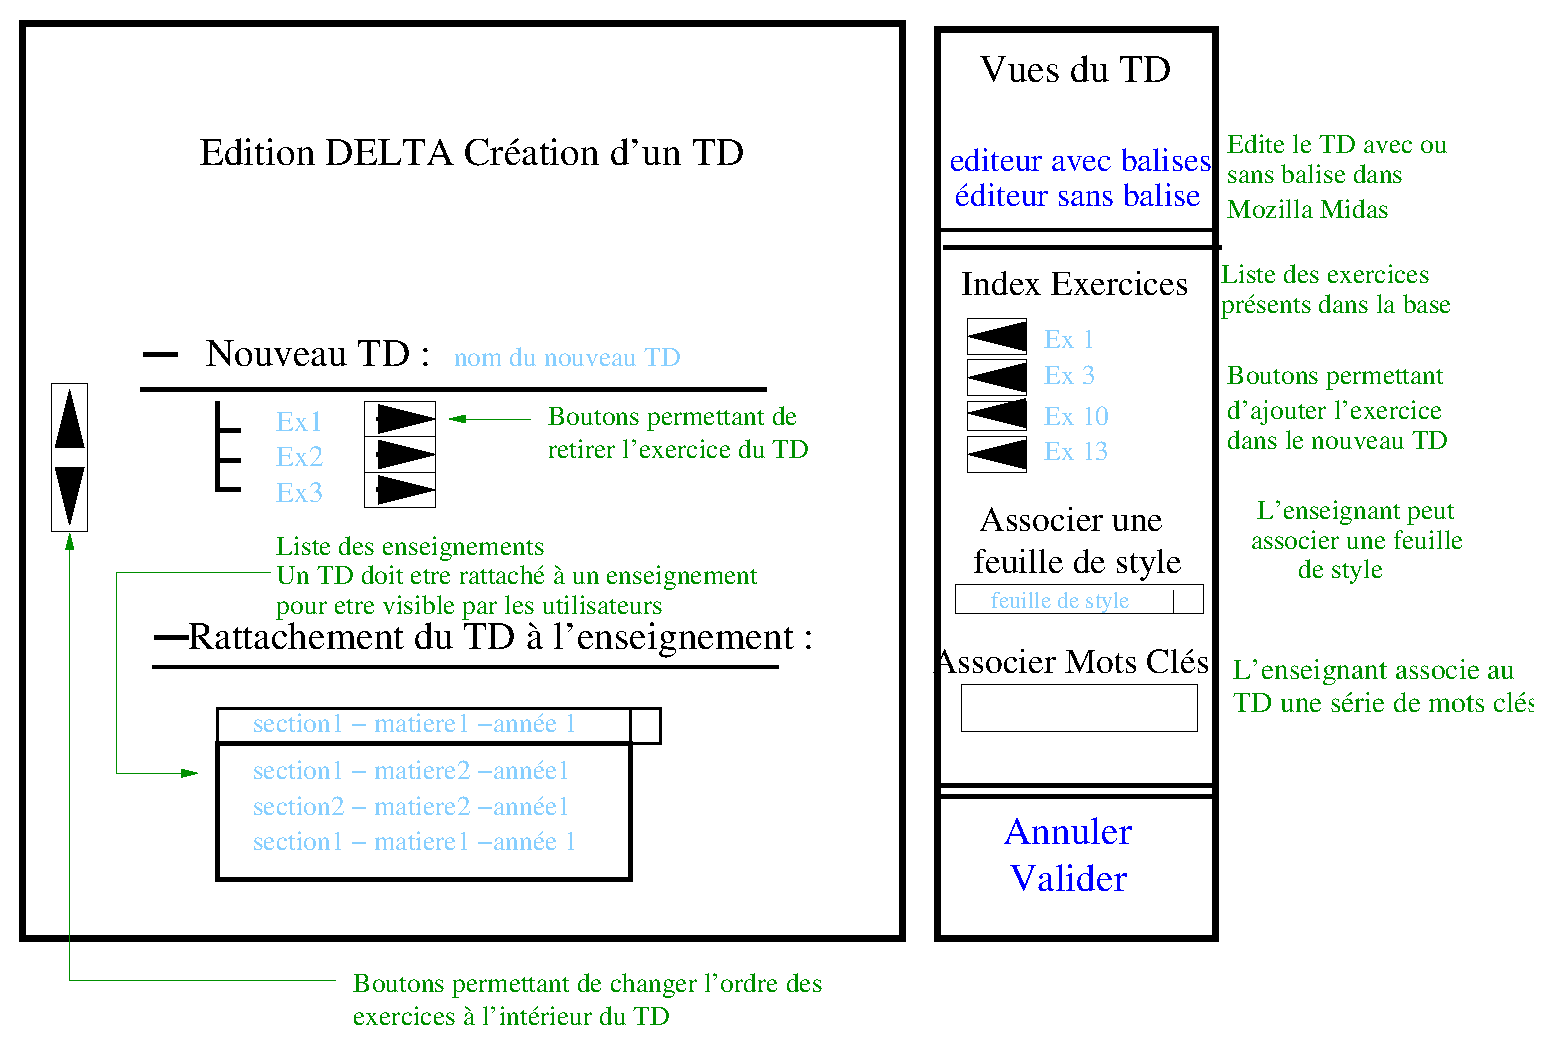
\includegraphics{../eps/tdCreerPanier.eps}}\\
{\it Vue Delta}
\end{flushleft}

L'enseignant enregistre son TD.

\section{Feuille de style}
Les TD et projets ont un formatage par d�faut (configur� par l'administrateur).
Lors de la cr�ation d'un TD ou projet, l'enseignant a la possiblit� de
formater ces derniers. 
\begin{flushleft}
\scalebox{0.5}{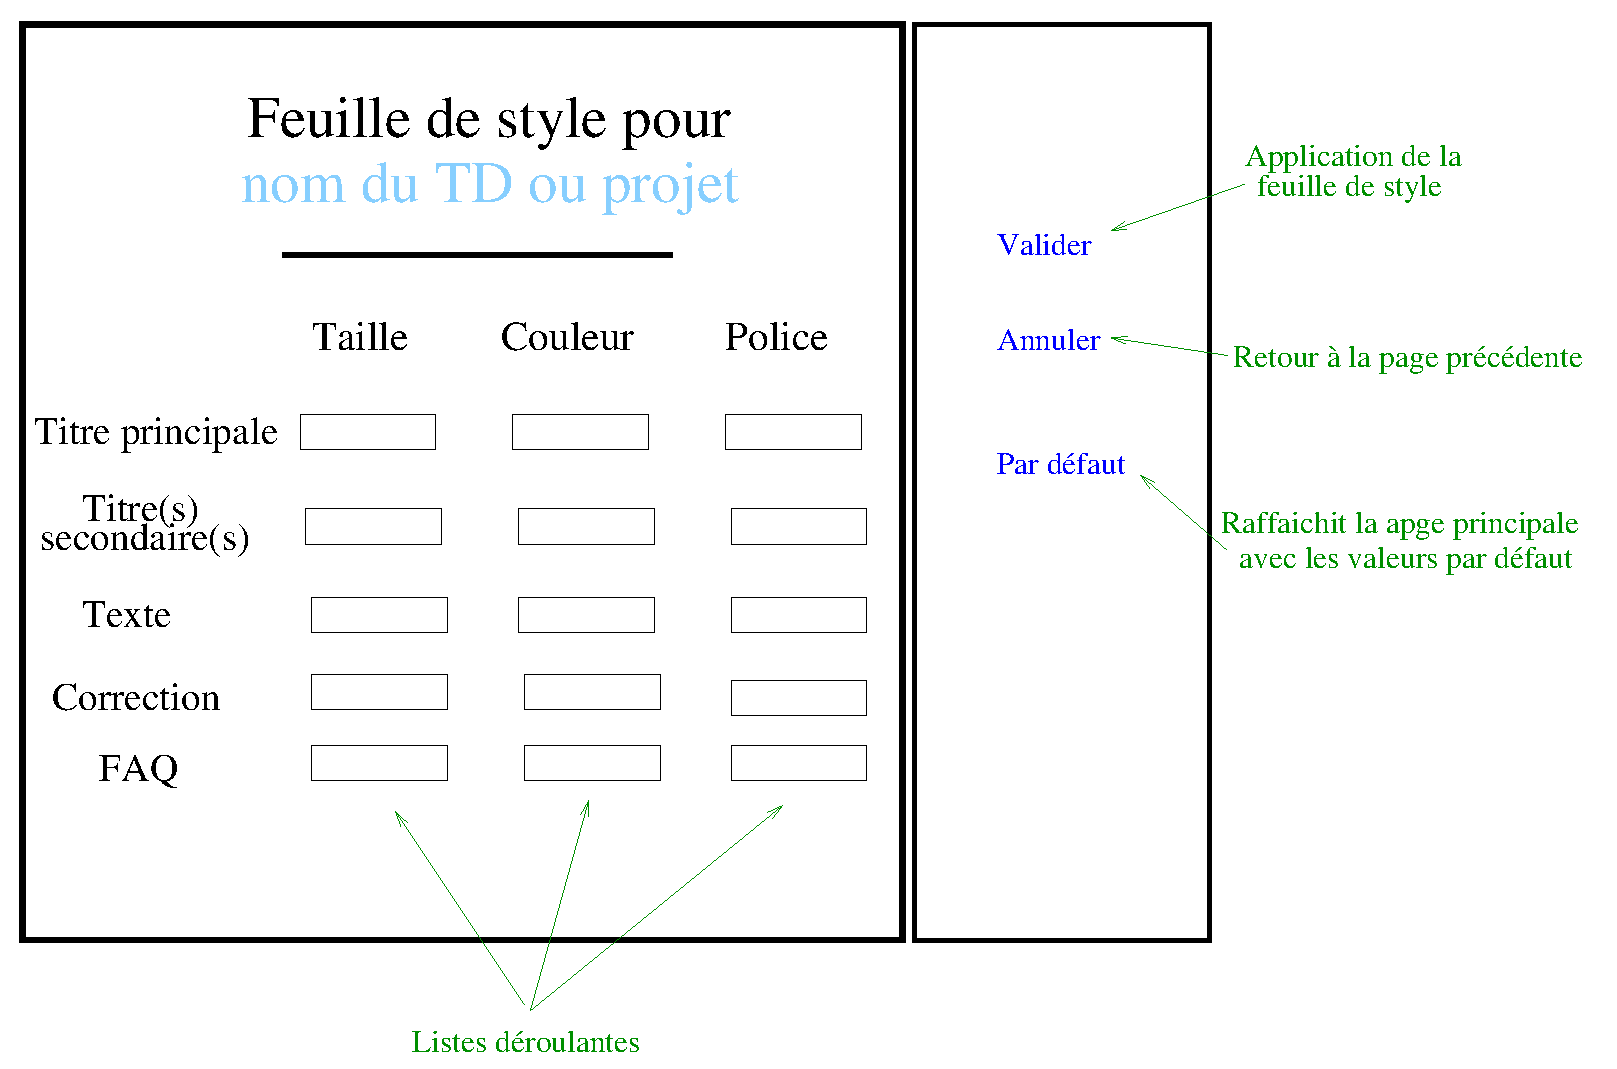
\includegraphics{../eps/feuilleDeStyle.eps}}\\
{\it La page de formatage est la m�me pour les TD et projets}
\end{flushleft}
La page d'application d'une feuille de style comporte des listes
d�roulantes, ce qui facilite les choix, et s'applique pour chaque
projet et TD.




\section{Cr�er un exercice}
\subsection{Page principale}
Nous allons d�tailler dans cette partie le sc�nario de cr�ation d'un exercice.
L'enseignant cr�er un exercice en cliquant sur le lien "Cr�er un exercice" dans la zone de lien.
Il existe deux mani�res de cr�er un exercice:
\begin{itemize}
\item Soit il reprend un exercice qui existe dans la base : lien {\it � partir d'un exercice existant dans la base}
\item Soit il en cr�e un nouveau : lien {\it un nouvel exercice}
\end{itemize}
	
\begin{flushleft}
\scalebox{0.5}{\includegraphics{../eps/exercice.eps}}\\
{\it Page principale}
\end{flushleft}

\subsection{A partir d'un ancien}
\begin{flushleft}
\scalebox{0.5}{\includegraphics{../eps/exerciceList.eps}}\\
{\it L'enseignant doit s�lectionner un exercice dans la base.
Il s�lectionne l'exercice dans le navigateur.}
\end{flushleft}

\subsection{Nouvel exercice}
Il existe deux mani�res de cr�er un nouvel exercice:
\begin{itemize}
\item Soit l'enseignant importe un fichier XML depuis son compte.
\item Soit il �dite directement l'exercice dans l'�diteur de bord.
\end{itemize}
\begin{flushleft}
\scalebox{0.5}{\includegraphics{../eps/exerciceNouveau.eps}}\\
{\it Cr�ation d'un nouvel exercice}
\end{flushleft}

\subsection{Import}
\begin{flushleft}
\scalebox{0.5}{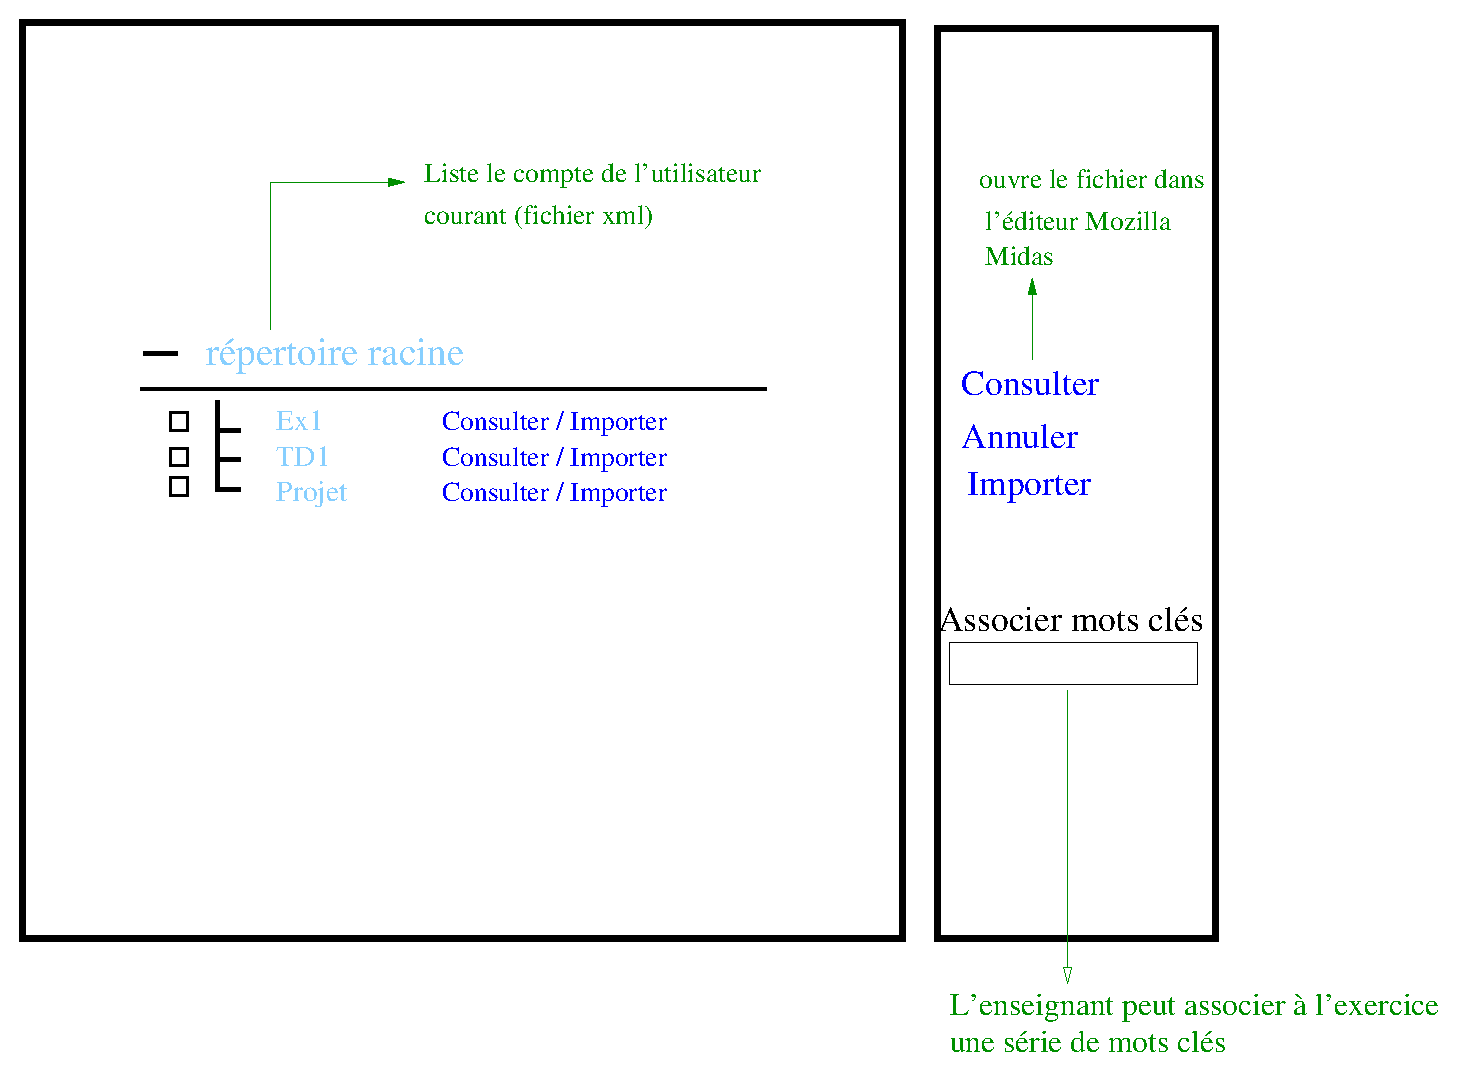
\includegraphics{../eps/exerciceExplorCompte.eps}}\\
{\it Listing du compte de l'utilisateur pour l'import}
\end{flushleft}

\subsection{Editeur de bord avec/sans balise XML}
L'�diteur de bord permet la saisie de l'exercice avec ou sans balise.

L'enseignant utilise pour la saisie de l'exercice l'�diteur embarqu�, dans la zone de visualisation.

Il existe deux mani�res d'�crire l'exercice.
\begin{flushleft}
\scalebox{0.5}{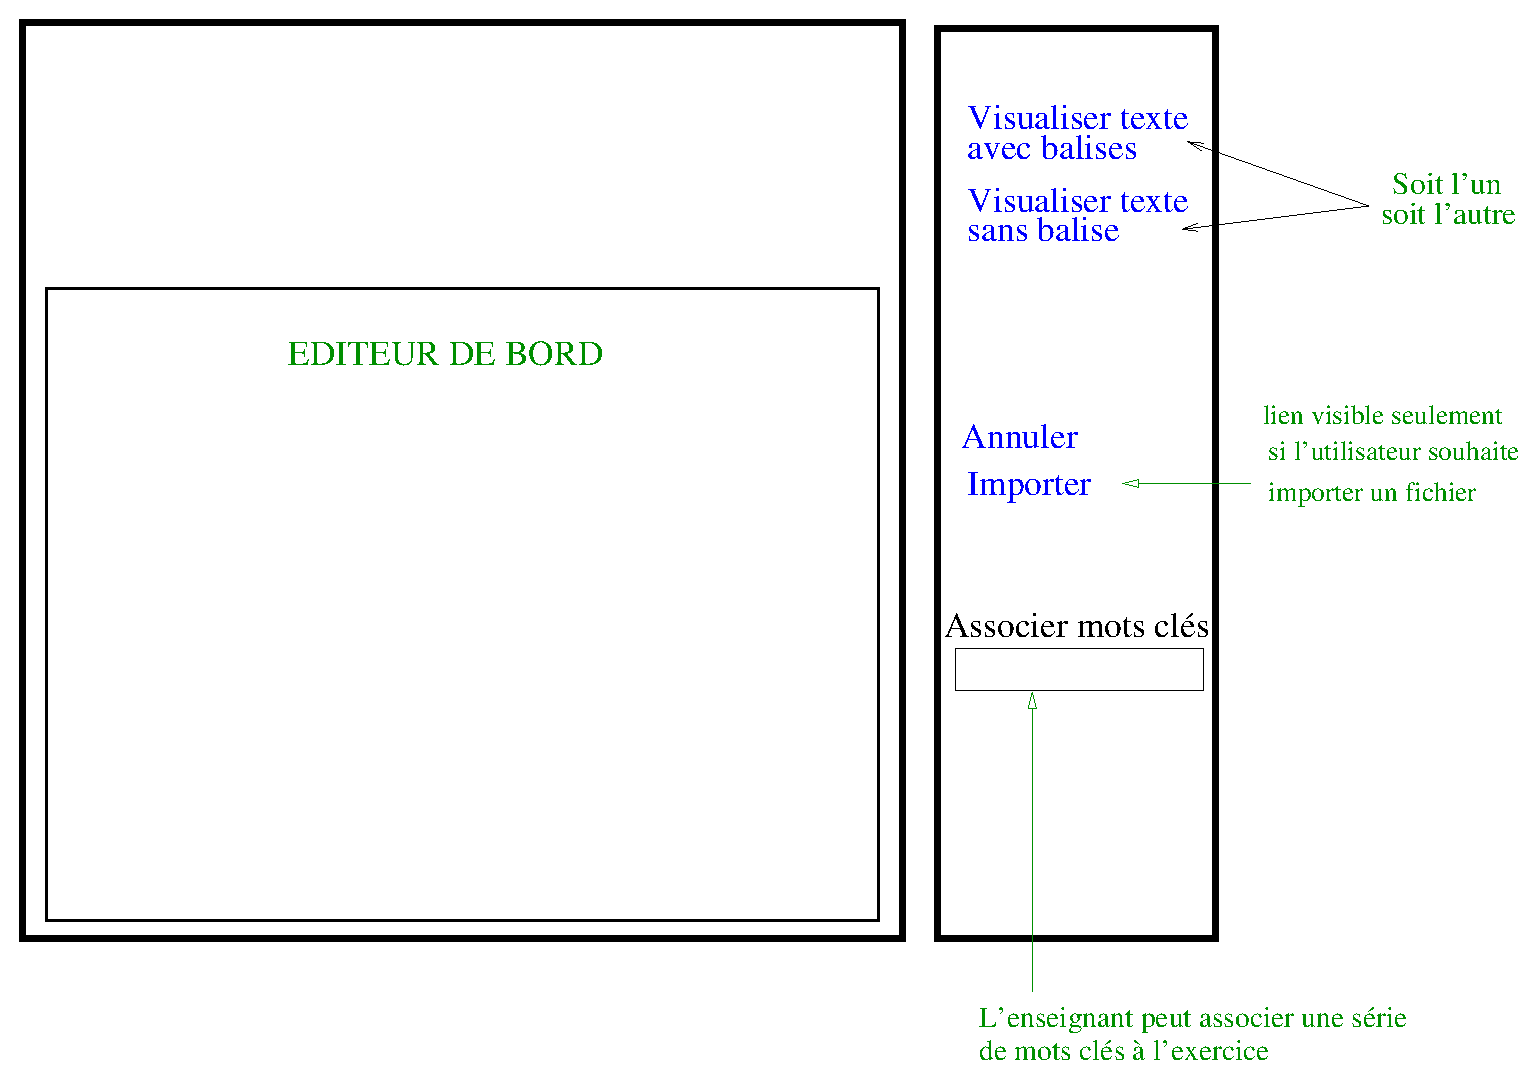
\includegraphics{../eps/exerciceEditText.eps}}\\
{\it L'enseignant saisie l'exercice directement en XML ou sans balise
selon le mode s�lectionn�}
\end{flushleft}



\section{Cr�er un enseignement}

\begin{flushleft}
Un enseignant peut cr�er un nouvel enseignement. 
Il devient alors responsable de cet enseignement.\\
Un enseignement est caract�ris� par une section - une mati�re - une ann�e
(ex : Maitrise - Genie Logiciel - 2003)
L'enseignant doit renseigner ces trois champs pour cr�er une enseignement.
Pour �viter les cr�ations multiples de mati�res (ex :maths
math�matiques ...), on met � disposition un module une saisie des donn�es semi-automatique, c'est-�-dire que lorsque l'utilisateur saisit les
diff�rents champs, l'application essaie de compl�ter avec des noms
existants dans la base. Cela facilite ainsi la tache �
l'utilisateur.\\
De plus, une liste d�roulante est associ� � chaque champ. Ces listes
contiennent l'ensemble des sections (si on est dans le champ section)
tri�s par ordre alphab�tique, ce qui permet encore une fois une saisie
rapide et ais� pour l'utilisateur. 

\scalebox{0.5}{\includegraphics{../eps/enseignementMain.eps}}\\
{\it Page principale de la cr�ation d'un enseignement}
\end{flushleft}


Pour cr�er l'enseignement l'enseignant clique sur le lien "valider".
La page suivante indique l'enseignement cr�er.
\begin{flushleft}
\scalebox{0.5}{\includegraphics{../eps/enseignementOK.eps}}\\
{\it Cr�ation r�ussie}
\end{flushleft}


Si il y a eu une erreur lors de la saisie des renseignements, un message d'erreur apparait.
\begin{flushleft}
\scalebox{0.5}{\includegraphics{../eps/enseignementNOK.eps}}\\
{\it Cr�ation �chou�e}
\end{flushleft}











\section{Cr�er un compte}

Lorsque l'administrateur souhaite ajouter de nouveaux enseignants, il
se dirige vers la page de cr�ation du compte � l'aide des liens qu'il
dispose dans la zone de liens.\\
Les champs {\it Nom} et {\it Pr�nom} sont des champs obligatoires car
ils sont n�cesssaires � la cr�ation automatique des logins et mots de
passe, ce qui retire � l'administrateur une lourde tache.  
\begin{flushleft}
\scalebox{0.5}{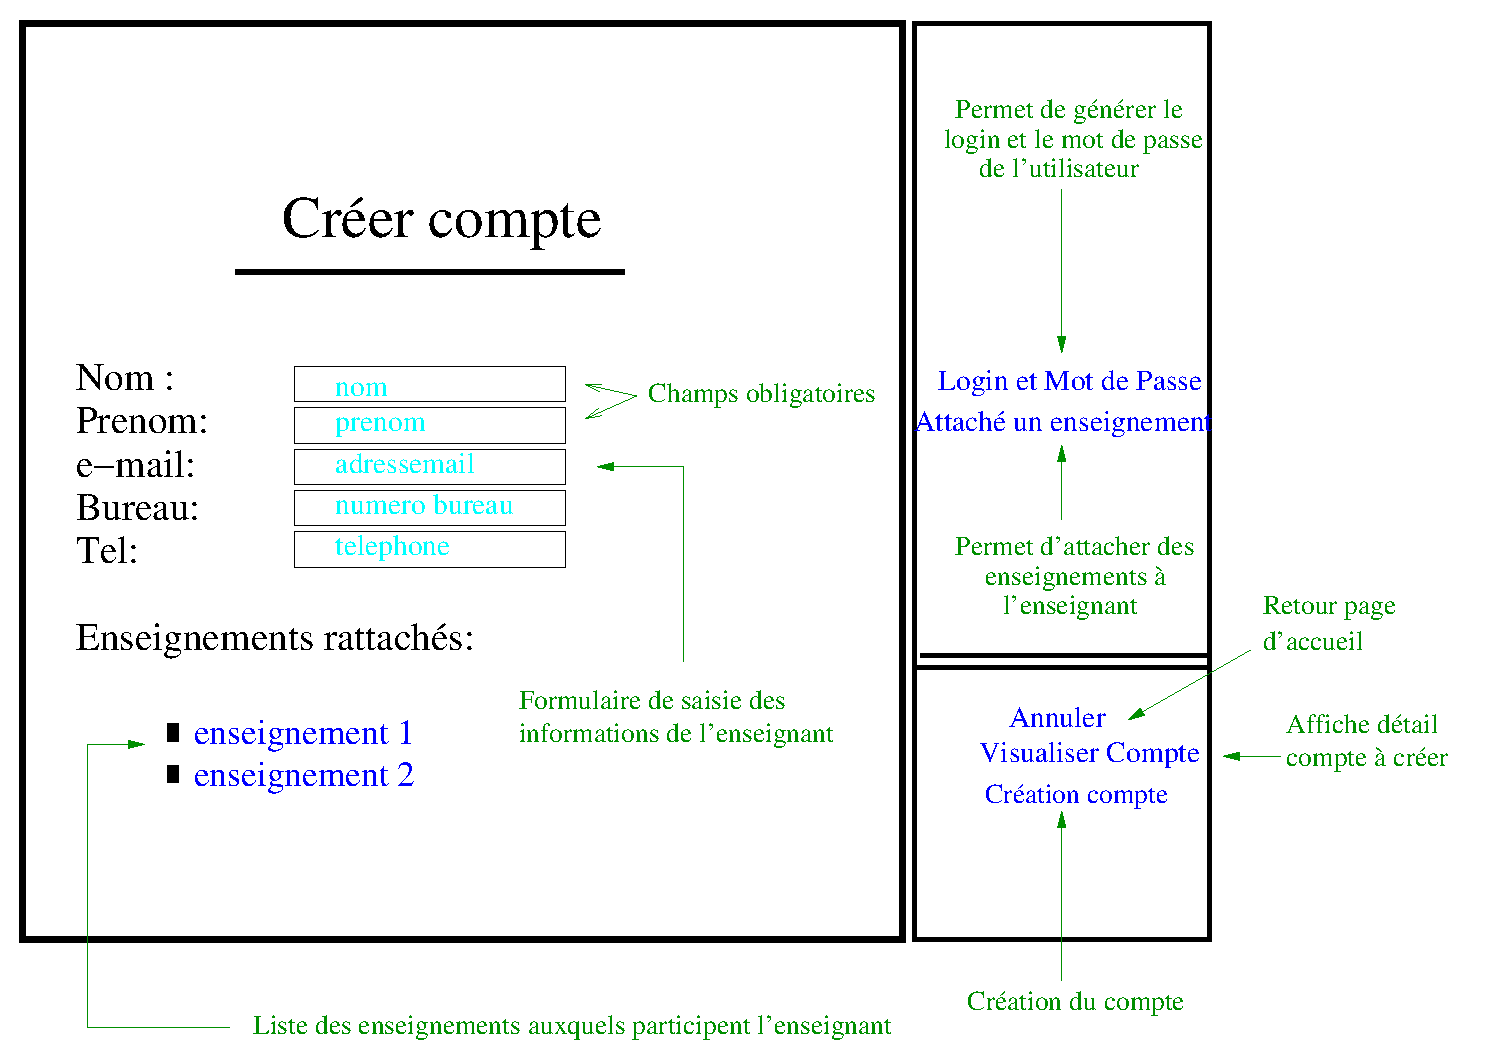
\includegraphics{../eps/compteCreer.eps}}\\
{\it Fen�tre de cr�ation du compte}
\end{flushleft}

L'administrateur a la possiblit� de valider � la cr�ation du compte
mais �galement d'avoir un aper�u du compte.
\begin{flushleft}
\scalebox{0.5}{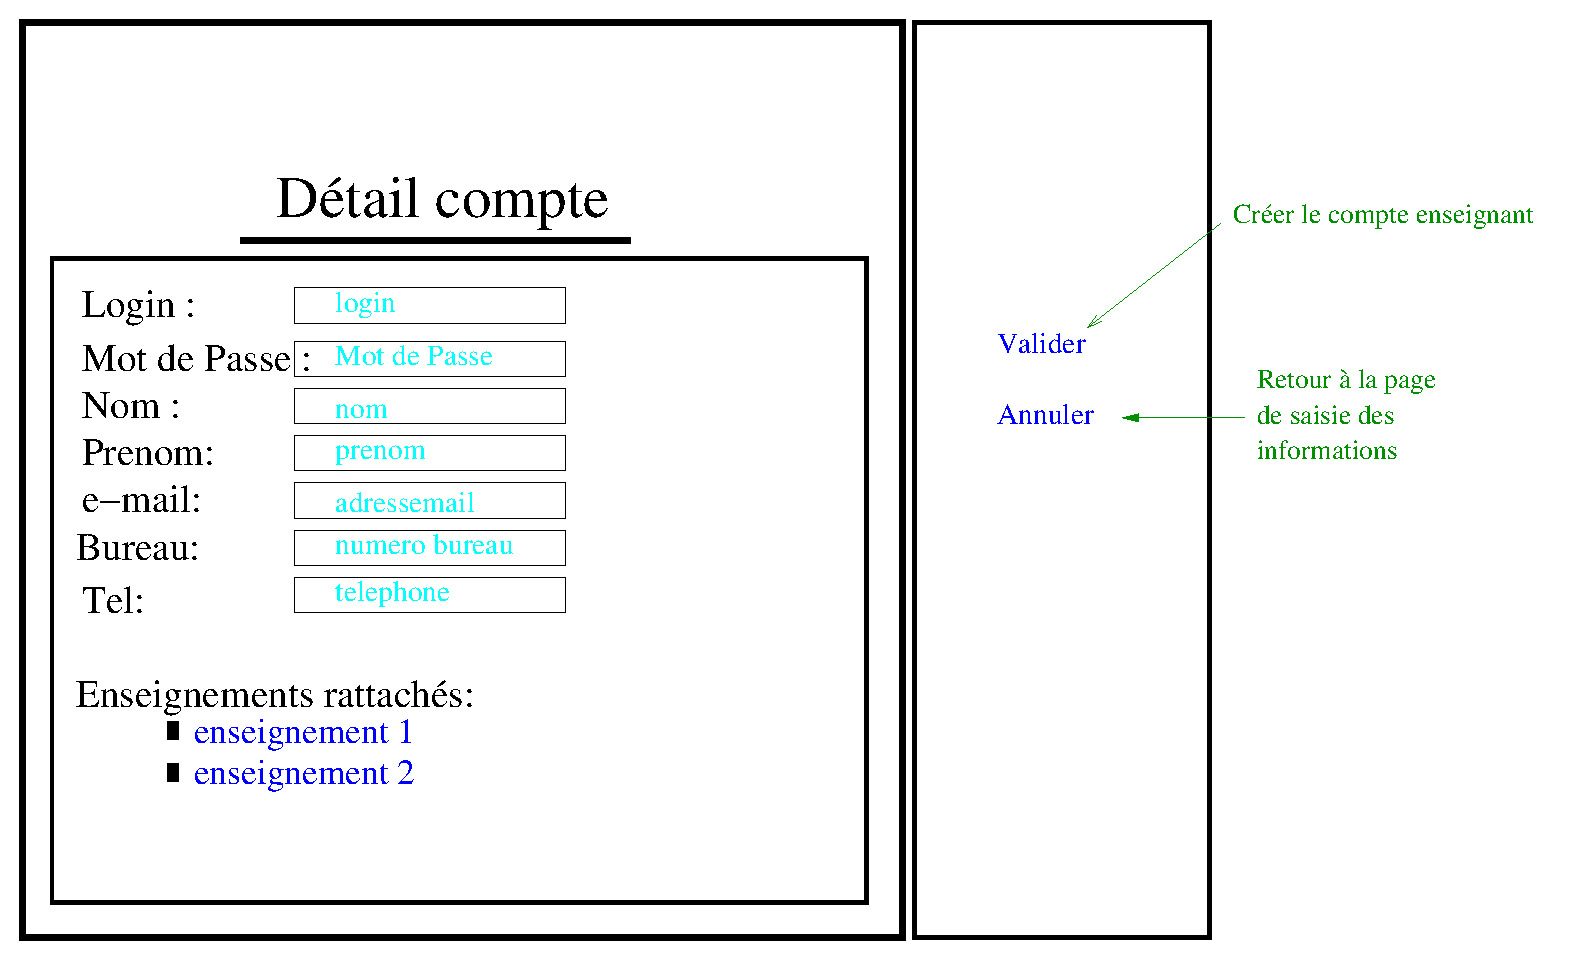
\includegraphics{../eps/compteDemandeConf.eps}}\\
{\it Visualisation du compte avant validation}
\end{flushleft}




	
\section{La corbeille}
La corbeille est un dernier lieu de stockage des donn�es effac�es par
les enseignants et m�me l'administrateur. Cette zone, seulement
accessible par l'administrateur de l'application, permet soit une
suppression d�finitive des donn�es soit une restauration.\\
De plus, pour faciliter sa consultation, la corbeille permet plusieurs
affichages. 

\begin{flushleft}
\scalebox{0.5}{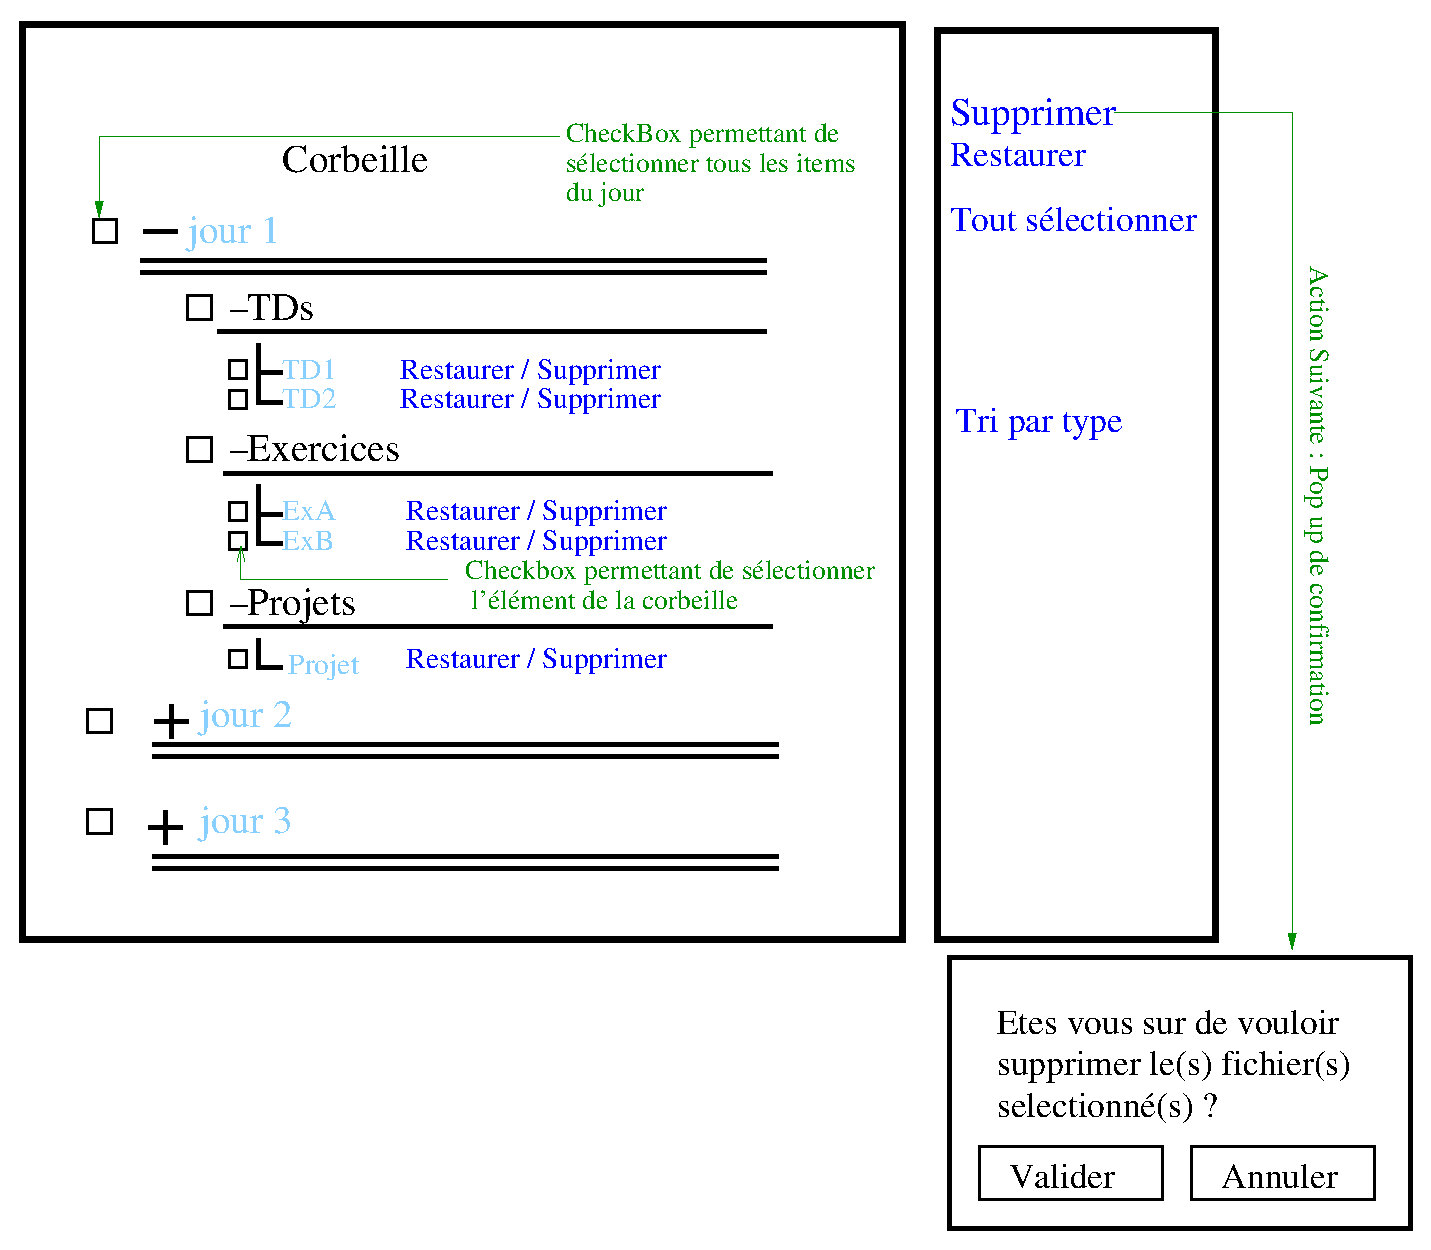
\includegraphics{../eps/corbeilleTriDate.eps}}\\
{\it Corbeille tri� par date}
\end{flushleft}

\begin{flushleft}
\scalebox{0.5}{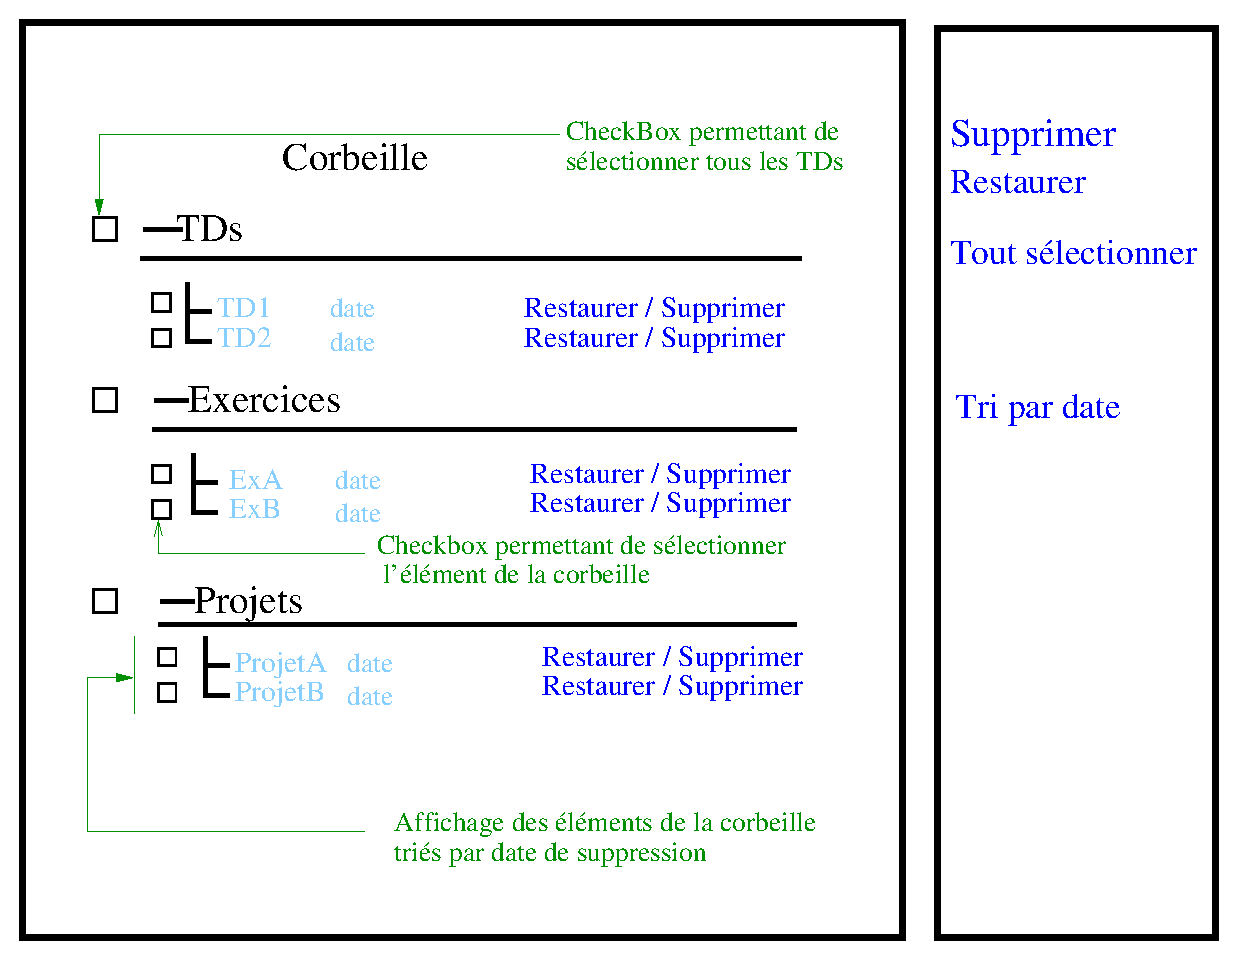
\includegraphics{../eps/corbeilleTriType.eps}}\\
{\it Corbeille tri� par type}
\end{flushleft}


La corbeille permet de restaurer les donn�es s�lectionn�es par
l'administrateur. L'application offre la possibilit� de s�lectionner
certains �lements ou un groupe d'�l�ments. 
\begin{flushleft}
\scalebox{0.5}{\includegraphics{../eps/corbeilleListRestaur.eps}}\\
{\it Corbeille apr�s restauration}
\end{flushleft}




\chapter{Planning pr�visionnel}

Ci-dessous, l'�tat d'avancement du projet et le planning pr�visionnel.\\

\begin{center}
\scalebox{0.5}{\includegraphics{images/exemple3.jpg}}\\
\par{Planning pr�visionnel}
\end{center}

\section*{Contacts}

Pour toutes questions compl{\'e}mentaires veuillez vous adresser {\`a} l'une
des personnes suivantes :\\

\begin{tabular}{|l|l|}
\hline
Nom & Email \\
\hline
Batoussa MOUGAMADOU & bat\_fr@hotmail.com\\
\hline
Saliou NGOM & sngom@mailcity.com\\
\hline
Vincent BOISSIN & vboissin@etudiant.univ-mlv.fr\\
\hline
Gabriel DUPONT & gdupont@etudiant.univ-mlv.fr\\
\hline
Julien KIRSCH & jkirsch@etudiant.univ-mlv.fr\\
\hline
Frederic GARCIA & fgarci01@etudiant.univ-mlv.fr\\
\hline
\end{tabular}



\end{document}




